% Place the text of this subsection here
A first element common to most science communications is figures. The code block bellow these lines inside \texttt{results\_subsection\_1.tex} inserts Figure~\ref{fig:ex}, showing how basic usage of this feature works in LaTeX. 

% Figure insertion example
\begin{figure}[ht]
    \centering
    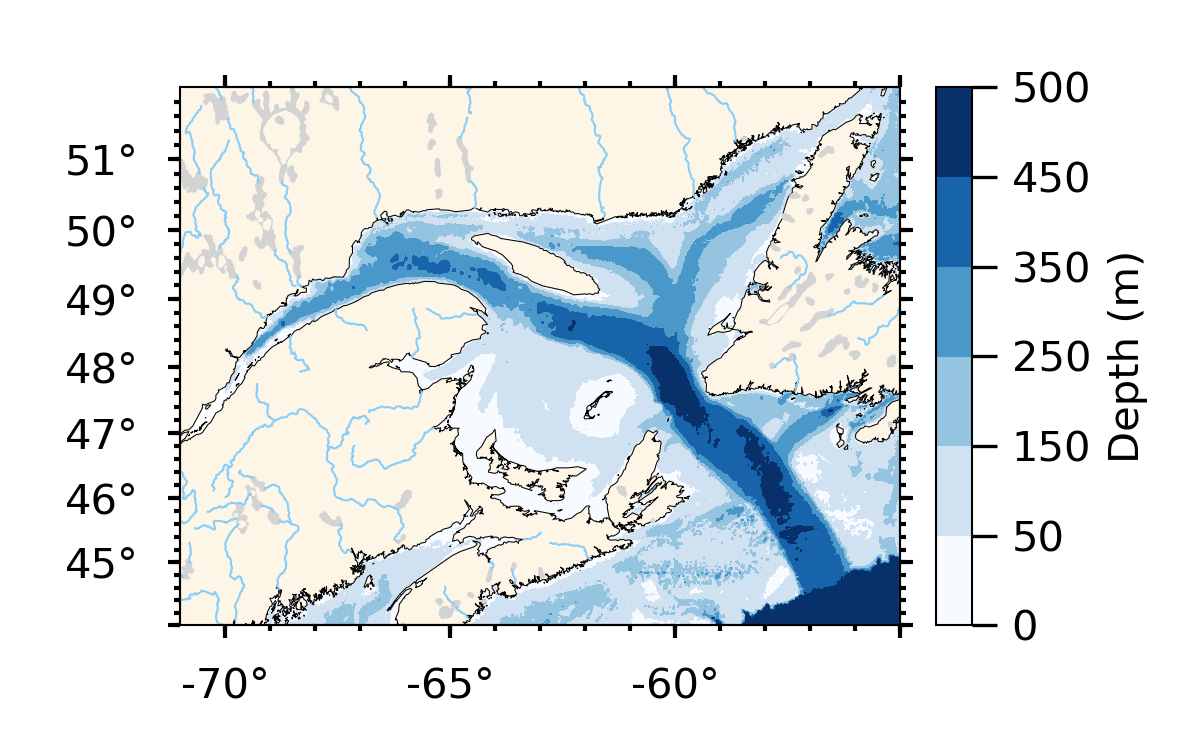
\includegraphics[width=0.75\linewidth]{figures/gsl_bathymetry_gebco.png}
    \caption{An example to illustrate the inclusion of figures to this template. Note that it does not appear where this block of code is written but rather at the location LaTeX deems most convenient, close to where it is first referenced.}
    \label{fig:ex}
\end{figure}

Some reports also require equations. The code inserting Equation~\ref{eq:average} can also be found in \texttt{results\_subsection\_1.tex} and exemplifies several useful notation elements such as fractions, indices and greek letters. For more information consult the Wikipedia page for LaTeX mathematics.

% Equation example
\begin{equation}
    \mu = \frac{1}{n}\sum_{i=0}^{n}x_i
    \label{eq:average}
\end{equation}

\noindent
Briefer mathematical statements can be inserted inline using the \$\$ notation, for example $\mu \neq 0$.